\subsubsection{Optimal Learning Rate}
\label{sec:improving-performance-learning-rate}
The learning rate is the most important hyperparameter in a neural network.
If it is too small, learning converges exactly, though, really slow.
If it is too large, the minimum is steadily overshot and learning maybe diverges.

\textit{Smith} introduces the cyclical learning rate \cite{DBLP:journals/corr/Smith15a}.
For being cyclical, the learning rate needs a lower and upper bound.
This builds a range of optimal learning rates.
With these values in between, the evaluations of the cost function are effectively decreased over time.
Hence, for finding that optimal range, the learning rate is initialized with a very small value and slightly increased after each training step.
For each of the steps the cost function is evaluated.
\figref{fig:optimal-learning-rate-range} shows a typical plot of the cost function against the learning rate on a logarithmic $x$-scale.
\begin{figure}
	\setlength\figureheight{.45\textwidth}
	\setlength\figurewidth{.9\textwidth}
	\centering
	% This file was created by matplotlib2tikz v0.7.3.
\begin{tikzpicture}

\begin{axis}[
height=\figureheight,
log basis x={10},
tick align=outside,
tick pos=left,
width=\figurewidth,
x grid style={white!69.01960784313725!black},
xlabel={Learning Rate},
xmin=4.84550334060697e-07, xmax=4.05399428541478,
xmode=log,
xtick style={color=black},
xtick={1e-08,1e-07,1e-06,1e-05,0.0001,0.001,0.01,0.1,1,10,100},
xticklabels={,,\(\displaystyle {10^{-6}}\),\(\displaystyle {10^{-5}}\),\(\displaystyle {10^{-4}}\),\(\displaystyle {10^{-3}}\),\(\displaystyle {10^{-2}}\),\(\displaystyle {10^{-1}}\),\(\displaystyle {10^{0}}\),,},
y grid style={white!69.01960784313725!black},
ylabel={Loss},
ymin=0.338506191968918, ymax=2.88608637452126,
ytick style={color=black}
]
\draw [fill=blue, draw opacity=0, fill opacity=0.2]
       (0.02,0) rectangle (0.2,3);
\addplot [semithick, green!50.0!black]
table {%
9.99999997475243e-07 2.42450165748596
1.0500000371394e-06 2.42557811737061
1.10250005036505e-06 2.42596864700317
1.1576250926737e-06 2.42507457733154
1.21550635867607e-06 2.42593574523926
1.27628163681948e-06 2.42624926567078
1.34009576413519e-06 2.42431640625
1.40710051255155e-06 2.42626357078552
1.47745549838874e-06 2.425452709198
1.55132829604554e-06 2.42539739608765
1.62889466537308e-06 2.42454528808594
1.71033934748266e-06 2.42561554908752
1.79585629211942e-06 2.42605042457581
1.88564911240974e-06 2.42541933059692
1.97993153960851e-06 2.42513751983643
2.07892821890709e-06 2.4241042137146
2.1828745957464e-06 2.42664480209351
2.29201828005898e-06 2.42587995529175
2.40661915995588e-06 2.42547607421875
2.52695008384762e-06 2.42530512809753
2.65329754256527e-06 2.42584633827209
2.78596235148143e-06 2.42603540420532
2.92526056000497e-06 2.42615008354187
3.07152367895469e-06 2.42545294761658
3.22509981742769e-06 2.42507410049438
3.38635481966776e-06 2.42465615272522
3.55567249243904e-06 2.42426776885986
3.73345619664178e-06 2.42627573013306
3.92012907468597e-06 2.42673063278198
4.11613564210711e-06 2.42567133903503
4.3219424696872e-06 2.42607235908508
4.5380397750705e-06 2.42514038085938
4.76494187751086e-06 2.42572379112244
5.00318901686114e-06 2.42429566383362
5.25334826306789e-06 2.42494058609009
5.51601578990812e-06 2.42493629455566
5.79181642024196e-06 2.42516303062439
6.08140726399142e-06 2.42453551292419
6.38547771814046e-06 2.42495155334473
6.70475174047169e-06 2.4251184463501
7.03998921380844e-06 2.42468881607056
7.39198867449886e-06 2.42531180381775
7.76158776716329e-06 2.425861120224
8.1496673374204e-06 2.42493557929993
8.55715097713983e-06 2.42545771598816
8.98500820767367e-06 2.42437195777893
9.43425857258262e-06 2.42548322677612
9.90597163763596e-06 2.42514276504517
1.04012706287904e-05 2.42492294311523
1.09213342511794e-05 2.425213098526
1.14674012365867e-05 2.42408061027527
1.20407712529413e-05 2.42323327064514
1.26428094517905e-05 2.42469072341919
1.3274950106279e-05 2.42428874969482
1.39386975206435e-05 2.4256796836853
1.46356323966756e-05 2.42457437515259
1.53674136527115e-05 2.42497706413269
1.61357838805998e-05 2.42544269561768
1.69425729836803e-05 2.42497372627258
1.77897018147632e-05 2.42535424232483
1.86791876330972e-05 2.42542028427124
1.96131477423478e-05 2.4250328540802
2.05938049475662e-05 2.42497944831848
2.16234948311467e-05 2.42398619651794
2.27046693908051e-05 2.42507195472717
2.38399024965474e-05 2.42351746559143
2.50318971666275e-05 2.42360186576843
2.62834928435041e-05 2.42472910881042
2.75976672128309e-05 2.42487645149231
2.89775507553713e-05 2.42378330230713
3.04264285659883e-05 2.42411494255066
3.19477512675803e-05 2.42305159568787
3.35451404680498e-05 2.42489814758301
3.52223978552502e-05 2.42497801780701
3.69835179299116e-05 2.42385292053223
3.88326952815987e-05 2.42340683937073
4.07743282266892e-05 2.42365145683289
4.28130442742258e-05 2.42285776138306
4.49536964879371e-05 2.42350673675537
4.72013816761319e-05 2.42474007606506
4.95614513056353e-05 2.42382860183716
5.20395224157255e-05 2.42289566993713
5.46414994460065e-05 2.42474460601807
5.73735742364079e-05 2.4228310585022
6.02422514930367e-05 2.42388868331909
6.32543669780716e-05 2.4234037399292
6.64170875097625e-05 2.42289423942566
6.973794370424e-05 2.42274522781372
7.32248445274308e-05 2.42197918891907
7.68860845710151e-05 2.42143750190735
8.07303877081722e-05 2.4215395450592
8.47669070935808e-05 2.42189192771912
8.90052542672493e-05 2.42235159873962
9.34555137064308e-05 2.42333054542542
9.81282864813693e-05 2.42215633392334
0.000103034697531257 2.42085838317871
0.000108186432044022 2.42255878448486
0.000113595757284202 2.42013835906982
0.000119275544420816 2.42067551612854
0.000125239326735027 2.41973280906677
0.000131501292344183 2.42023992538452
0.000138076356961392 2.41976165771484
0.00014498017844744 2.4191427230835
0.000152229185914621 2.42016816139221
0.000159840652486309 2.41934823989868
0.00016783268074505 2.41783905029297
0.000176224319147877 2.41864109039307
0.000185035532922484 2.41829085350037
0.000194287305930629 2.41694355010986
0.000204001669771969 2.41789174079895
0.000214201747439802 2.41790008544922
0.000224911840632558 2.41568660736084
0.000236157429753803 2.41686511039734
0.000247965304879472 2.4138355255127
0.000260363565757871 2.41464638710022
0.000273381738224998 2.41349053382874
0.00028705081786029 2.41510844230652
0.000301403371850029 2.41320371627808
0.000316473538987339 2.41130495071411
0.000332297204295173 2.41221141815186
0.000348912057233974 2.41114687919617
0.000366357649909332 2.41115498542786
0.00038467554259114 2.40984988212585
0.00040390933281742 2.41024422645569
0.000424104800913483 2.40897130966187
0.000445310026407242 2.40830111503601
0.00046757553354837 2.40786671638489
0.000490954320412129 2.40619421005249
0.000515502062626183 2.40558218955994
0.000541277171578258 2.40418243408203
0.000568341056350619 2.40358853340149
0.000596758094616234 2.40100359916687
0.000626595981884748 2.40136957168579
0.000657925789710134 2.39969801902771
0.000690822082106024 2.398592710495
0.000725363206584007 2.39649486541748
0.000761631352361292 2.39576411247253
0.000799712899606675 2.39480566978455
0.00083969853585586 2.39230513572693
0.0008816834888421 2.39280581474304
0.000925767642911524 2.38742923736572
0.000972056004684418 2.38858222961426
0.00102065876126289 2.38470411300659
0.00107169174589217 2.38383960723877
0.00112527632154524 2.38413643836975
0.00118154007941484 2.38072395324707
0.00124061712995172 2.37818050384521
0.0013026479864493 2.37578558921814
0.001367780379951 2.37448978424072
0.00143616937566549 2.37235426902771
0.00150797783862799 2.36923885345459
0.00158337678294629 2.36696767807007
0.0016625456046313 2.36402702331543
0.0017456728965044 2.36168217658997
0.00183295656461269 2.35784602165222
0.00192460441030562 2.35405468940735
0.00202083471231163 2.35085892677307
0.00212187645956874 2.34650373458862
0.0022279703989625 2.34306979179382
0.00233936891891062 2.34080719947815
0.00245633744634688 2.33668804168701
0.00257915421389043 2.33383584022522
0.00270811188966036 2.32863903045654
0.00284351757727563 2.32485318183899
0.00298569351434708 2.31907820701599
0.00313497823663056 2.31579113006592
0.0032917270436883 2.30975270271301
0.00345631339587271 2.30496621131897
0.00362912914715707 2.29987502098083
0.00381058570928872 2.29516816139221
0.00400111498311162 2.28918647766113
0.00420117052271962 2.28446960449219
0.00441122893244028 2.27698731422424
0.00463179033249617 2.27286696434021
0.00486337998881936 2.26446151733398
0.00510654877871275 2.25733041763306
0.00536187645047903 2.25242614746094
0.00562997022643685 2.2435348033905
0.00591146852821112 2.23614764213562
0.00620704190805554 2.22918653488159
0.00651739398017526 2.2192006111145
0.00684326374903321 2.21188473701477
0.00718542700633407 2.2036771774292
0.00754469819366932 2.19467115402222
0.00792193319648504 2.18411374092102
0.00831803027540445 2.17430639266968
0.00873393192887306 2.1644606590271
0.00917062815278769 2.15557456016541
0.00962915923446417 2.14502096176147
0.0101106176152825 2.13331723213196
0.0106161488220096 2.12060713768005
0.0111469561234117 2.10897183418274
0.0117043042555451 2.09853720664978
0.0122895194217563 2.08424425125122
0.0129039958119392 2.07019567489624
0.0135491956025362 2.05744338035583
0.0142266554757953 2.04196381568909
0.0149379884824157 2.02743220329285
0.0156848877668381 2.01219868659973
0.01646913215518 1.99649918079376
0.0172925889492035 1.9794842004776
0.0181572176516056 1.96140170097351
0.0190650783479214 1.94388604164124
0.0200183317065239 1.92706489562988
0.0210192482918501 1.90680551528931
0.0220702104270458 1.88815832138062
0.0231737215071917 1.86732268333435
0.024332407861948 1.84716463088989
0.0255490280687809 1.8243362903595
0.0268264785408974 1.80285751819611
0.0281678028404713 1.77907490730286
0.0295761935412884 1.75590872764587
0.0310550034046173 1.73087549209595
0.0326077528297901 1.70459842681885
0.0342381410300732 1.68064713478088
0.0359500497579575 1.65356779098511
0.0377475507557392 1.62749409675598
0.0396349281072617 1.59828794002533
0.0416166745126247 1.5703729391098
0.0436975099146366 1.54173922538757
0.0458823852241039 1.51172959804535
0.0481765046715736 1.48154401779175
0.0505853295326233 1.45072913169861
0.0531145967543125 1.41898798942566
0.0557703264057636 1.38806974887848
0.0585588440299034 1.35568904876709
0.0614867880940437 1.32473230361938
0.064561128616333 1.29352927207947
0.0677891820669174 1.26147782802582
0.0711786448955536 1.22979140281677
0.0747375786304474 1.19731819629669
0.0784744545817375 1.1670788526535
0.0823981761932373 1.13524603843689
0.0865180864930153 1.10442161560059
0.090843990445137 1.07477796077728
0.0953861922025681 1.04593074321747
0.100155502557755 1.01714849472046
0.105163276195526 0.989579856395721
0.110421441495419 0.95998626947403
0.115942515432835 0.932793796062469
0.121739640831947 0.909042358398438
0.127826616168022 0.882031440734863
0.134217947721481 0.857464849948883
0.140928849577904 0.833971858024597
0.147975295782089 0.812260031700134
0.155374065041542 0.78940612077713
0.163142770528793 0.768466532230377
0.171299904584885 0.748415589332581
0.179864898324013 0.728718996047974
0.188858136534691 0.710050821304321
0.198301047086716 0.692308008670807
0.208216100931168 0.675094485282898
0.218626901507378 0.659027099609375
0.229558244347572 0.6426842212677
0.241036161780357 0.628868222236633
0.253087967634201 0.612840294837952
0.265742361545563 0.598800778388977
0.279029488563538 0.587084591388702
0.292980968952179 0.572641611099243
0.307630002498627 0.561109185218811
0.323011517524719 0.549902498722076
0.339162081480026 0.538087785243988
0.356120198965073 0.52801376581192
0.373926222324371 0.516906917095184
0.392622530460358 0.513492465019226
0.412253648042679 0.519908845424652
0.432866334915161 0.600372016429901
0.454509645700455 0.922281920909882
0.47723513841629 1.45273172855377
0.501096904277802 1.43346238136292
0.526151776313782 1.12832844257355
0.552459359169006 0.799192786216736
0.580082297325134 0.592928409576416
0.609086394309998 0.533975541591644
0.639540731906891 0.52020388841629
0.671517789363861 0.538137018680573
0.705093681812286 0.618704676628113
0.740348339080811 0.723499596118927
0.777365744113922 0.728213131427765
0.816234052181244 0.512662887573242
0.857045769691467 0.463998764753342
0.899898052215576 0.454305291175842
0.944892942905426 0.499062687158585
0.992137610912323 0.654571890830994
1.04174447059631 1.10818409919739
1.09383165836334 1.16981542110443
1.14852321147919 1.64061462879181
1.20594942569733 1.29171586036682
1.26624691486359 1.17091405391693
1.32955920696259 1.09842658042908
1.3960372209549 1.2668833732605
1.46583902835846 1.22053277492523
1.5391309261322 1.32041847705841
1.61608743667603 1.91480886936188
1.69689178466797 1.35100698471069
1.78173637390137 1.12154793739319
1.87082314491272 1.11014807224274
1.96436429023743 2.77028727531433
};
\end{axis}

\end{tikzpicture}
	\caption[Optimal range of learning rates]{Optimal range of learning rates highlighted in blue. The learning rate is increased exponentially.}
	\label{fig:optimal-learning-rate-range}
\end{figure}
It can be seen, that if the learning rate is small, the cost function does not improve noticeably.
When the learning rate gets into its optimal range, the cost function suddenly becomes smaller.
This continues with a large gradient until the learning rate exits its optimal range.
This passage is detected when the cost function starts to oscillate.
If the learning rate still gets increased, the cost function starts to diverge eventually.
\textit{Smith} suggests a triangular learning rate policy which first increases the learning rate from the lower bound to the upper bound and then decreases it back to the lower bound.
Each change happens linearly.
The actual learning rate depends on the time step.

Another approach is doing warm restarts of the learning rate after several iterations, hence, it is called Stochastic Gradient Descent with Warm Restarts \cite{DBLP:journals/corr/LoshchilovH16a}.
This is especially combined with the gradient descent algorithm.
The idea behind it is to swing out of a tight local minimum if the algorithm seems to get stuck there.
If well-suited parameters are found for a cost function, the latter can slightly change if the dataset changes.
Hence, the once well-suited parameters lead to a worse cost now.
Therefore, a minimum in a flatter region needs to be found where a slight change has no big impact, i.e. a solution that is more generalized across datasets.
\figref{fig:sgdr-cost} illustrates this scenario.
\begin{figure}
	\centering
	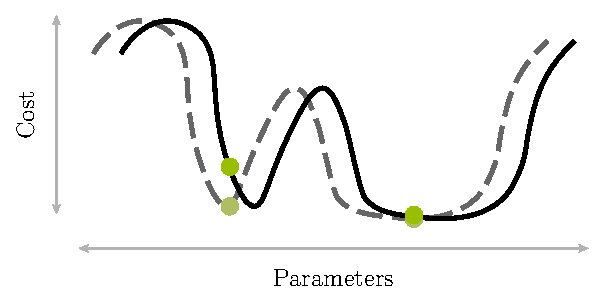
\includegraphics[]{images/sgdr-cost.pdf}
	\caption[Cost function of different datasets]{Cost function of different datasets. If the parameters represent a minimum of a dataset's cost function, the same parameters do not inevitably represent the minimum of a different dataset's cost function.}
	\label{fig:sgdr-cost}
\end{figure}
This algorithm uses a cosine annealing of the learning rate.
This means the learning rate is decreased in the form of half a cosine curve.
This is called a cycle.
After this, it is set to its initial value and the annealing is repeated.
This process is visualized in \figref{fig:sgdr-annealing-normal}.
\begin{figure}
	\setlength\figureheight{.3\textwidth}
	\setlength\figurewidth{.45\textwidth}
	\centering
	\begin{subfigure}{.49\textwidth}
		\centering
		% This file was created by matplotlib2tikz v0.7.4.
\begin{tikzpicture}

\begin{axis}[
height=\figureheight,
tick align=outside,
tick pos=left,
width=\figurewidth,
x grid style={white!90.01960784313725!black},
xlabel={Iterations},
xmajorgrids,
xmin=-47.2, xmax=991.2,
xtick style={color=black},
y grid style={white!90.01960784313725!black},
ylabel={Learning Rate},
ymajorgrids,
ymin=0.00500006658430417, ymax=0.114999996829319,
ytick style={color=black},
ytick={0.01,0.035,0.06,0.085,0.11},
yticklabels={0.01,,,,0.1}
]
\addplot [semithick, green!50.0!black]
table {%
0 0.11
1 0.109997500020833
2 0.109990000333329
3 0.109977501687449
4 0.109960005333049
5 0.109937513019748
6 0.10991002699676
7 0.109877550012664
8 0.109840085315131
9 0.1097976366506
10 0.109750208263901
11 0.109697804897835
12 0.109640431792693
13 0.109578094685739
14 0.109510799810632
15 0.109438553896802
16 0.109361364168781
17 0.109279238345478
18 0.109192184639406
19 0.109100211755864
20 0.109003328892062
21 0.108901545736207
22 0.10879487246653
23 0.108683319750269
24 0.108566898742601
25 0.108445621085532
26 0.108319498906726
27 0.108188544818295
28 0.108052771915539
29 0.107912193775635
30 0.10776682445628
31 0.107616678494286
32 0.107461770904122
33 0.107302117176419
34 0.107137733276417
35 0.106968635642369
36 0.106794841183897
37 0.106616367280302
38 0.106433231778826
39 0.106245452992866
40 0.106053049700144
41 0.10585604114083
42 0.105654447015615
43 0.105448287483744
44 0.105237583160998
45 0.105022355117634
46 0.104802624876276
47 0.104578414409766
48 0.104349746138964
49 0.104116642930506
50 0.103879128094519
51 0.103637225382288
52 0.103390958983882
53 0.103140353525738
54 0.102885434068191
55 0.102626226102975
56 0.102362755550671
57 0.102095048758113
58 0.101823132495759
59 0.101547033955008
60 0.101266780745484
61 0.100982400892274
62 0.100693922833127
63 0.100401375415608
64 0.100104787894215
65 0.0998041899274528
66 0.0994996115748683
67 0.0991910832940425
68 0.0988786359375464
69 0.0985623007498553
70 0.0982421093642244
71 0.0979180937995254
72 0.0975902864570447
73 0.0972587201172435
74 0.0969234279364794
75 0.096584443443691
76 0.0962418005370453
77 0.0958955334805472
78 0.0955456769006139
79 0.0951922657826118
80 0.0948353354673583
81 0.0944749216475873
82 0.0941110603643807
83 0.0937437880035634
84 0.0933731412920654
85 0.0929991572942491
86 0.0926218734082026
87 0.0922413273620001
88 0.091857557209929
89 0.0914706013286848
90 0.0910804984135332
91 0.0906872874744406
92 0.0902910078321731
93 0.0898916991143649
94 0.0894894012515549
95 0.0890841544731942
96 0.0886759993036228
97 0.0882649765580177
98 0.0878511273383109
99 0.0874344930290794
100 0.087015115293407
101 0.0865930360687178
102 0.0861682975625825
103 0.0857409422484978
104 0.0853110128616389
105 0.0848785523945863
106 0.0844436040930264
107 0.0840062114514267
108 0.083566418208687
109 0.083124268343765
110 0.0826798060712789
111 0.0822330758370853
112 0.0817841223138356
113 0.0813329903965079
114 0.0808797251979179
115 0.0804243720442079
116 0.0799669764703137
117 0.0795075842154115
118 0.0790462412183441
119 0.0785829936130266
120 0.0781178877238337
121 0.0776509700609665
122 0.0771822873158023
123 0.0767118863562251
124 0.0762398142219388
125 0.0757661181197634
126 0.0752908454189145
127 0.0748140436462659
128 0.0743357604815978
129 0.0738560437528279
130 0.0733749414312294
131 0.0728925016266335
132 0.0724087725826186
133 0.0719238026716862
134 0.071437640390423
135 0.0709503343546521
136 0.070461933294571
137 0.0699724860498786
138 0.0694820415648917
139 0.06899064888365
140 0.068498357145012
141 0.0680052155777416
142 0.0675112734955843
143 0.0670165802923368
144 0.0665211854369073
145 0.0660251384683683
146 0.0655284889910035
147 0.0650312866693466
148 0.0645335812232155
149 0.06403542242274
150 0.0635368600833851
151 0.0630379440609693
152 0.062538724246679
153 0.0620392505620795
154 0.0615395729541233
155 0.0610397413901546
156 0.0605398058529134
157 0.0600398163355367
158 0.0595398228365596
159 0.0590398753549154
160 0.0585400238849356
161 0.0580403184113506
162 0.0575408089042915
163 0.0570415453142926
164 0.0565425775672969
165 0.0560439555596633
166 0.055545729153177
167 0.0550479481700636
168 0.0545506623880064
169 0.0540539215351694
170 0.0535577752852238
171 0.0530622732523811
172 0.0525674649864318
173 0.0520733999677901
174 0.0515801276025461
175 0.0510876972175254
176 0.050596158055356
177 0.0501055592695445
178 0.0496159499195608
179 0.0491273789659318
180 0.0486398952653456
181 0.0481535475657663
182 0.0476683845015583
183 0.0471844545886239
184 0.046701806219551
185 0.0462204876587744
186 0.045740547037749
187 0.0452620323501369
188 0.0447849914470083
189 0.0443094720320559
190 0.0438355216568248
191 0.0433631877159577
192 0.0428925174424551
193 0.042423557902952
194 0.0419563559930116
195 0.0414909584324357
196 0.0410274117605923
197 0.0405657623317624
198 0.0401060563105042
199 0.0396483396670367
200 0.0391926581726429
201 0.0387390573950924
202 0.038287582694085
203 0.0378382792167145
204 0.0373911918929544
205 0.0369463654311644
206 0.0365038443136199
207 0.036063672792064
208 0.035625894883282
209 0.0351905543647001
210 0.0347576947700071
211 0.034327359384802
212 0.0338995912422646
213 0.0334744331188528
214 0.0330519275300244
215 0.0326321167259864
216 0.0322150426874694
217 0.0318007471215295
218 0.0313892714573782
219 0.0309806568422389
220 0.0305749441372327
221 0.030172173913292
222 0.0297723864471035
223 0.0293756217170807
224 0.028981919399366
225 0.028591318863863
226 0.0282038591702999
227 0.027819579064323
228 0.0274385169736227
229 0.0270607110040906
230 0.0266861989360088
231 0.0263150182202719
232 0.0259472059746424
233 0.0255827989800381
234 0.0252218336768549
235 0.0248643461613223
236 0.024510372181894
237 0.0241599471356729
238 0.0238131060648716
239 0.0234698836533081
240 0.0231303142229377
241 0.0227944317304204
242 0.0224622697637255
243 0.0221338615387728
244 0.0218092398961113
245 0.0214884372976346
246 0.0211714858233353
247 0.0208584171680967
248 0.0205492626385234
249 0.0202440531498108
250 0.0199428192226533
251 0.0196455909801927
252 0.0193523981450055
253 0.0190632700361309
254 0.0187782355661389
255 0.0184973232382389
256 0.0182205611434296
257 0.0179479769576899
258 0.0176795979392112
259 0.0174154509256717
260 0.0171555623315526
261 0.0168999581454968
262 0.0166486639277099
263 0.0164017048074042
264 0.0161591054802859
265 0.0159208902060857
266 0.0156870828061324
267 0.0154577066609712
268 0.0152327847080254
269 0.0150123394393029
270 0.0147963928991469
271 0.0145849666820315
272 0.0143780819304021
273 0.0141757593325615
274 0.013978019120601
275 0.0137848810683768
276 0.0135963644895334
277 0.0134124882355714
278 0.0132332706939631
279 0.0130587297863132
280 0.0128888829665671
281 0.0127237472192652
282 0.0125633390578446
283 0.0124076745229879
284 0.0122567691810187
285 0.0121106381223455
286 0.0119692959599524
287 0.0118327568279378
288 0.0117010343801013
289 0.0115741417885777
290 0.0114520917425205
291 0.0113348964468326
292 0.0112225676209459
293 0.0111151164976493
294 0.0110125538219658
295 0.0109148898500773
296 0.0108221343482997
297 0.0107342965921058
298 0.0106513853651981
299 0.0105734089586302
300 0.0105003751699777
301 0.0104322913025587
302 0.0103691641647031
303 0.0103110000690722
304 0.010257804832027
305 0.0102095837730469
306 0.0101663417141977
307 0.0101280829796491
308 0.0100948113952427
309 0.0100665302881093
310 0.010043242486336
311 0.0100249503186836
312 0.0100116556143536
313 0.0100033597028053
314 0.010000063413623
315 0.11
316 0.109997500020833
317 0.109990000333329
318 0.109977501687449
319 0.109960005333049
320 0.109937513019748
321 0.10991002699676
322 0.109877550012664
323 0.109840085315131
324 0.1097976366506
325 0.109750208263901
326 0.109697804897835
327 0.109640431792693
328 0.109578094685739
329 0.109510799810632
330 0.109438553896802
331 0.109361364168781
332 0.109279238345478
333 0.109192184639406
334 0.109100211755864
335 0.109003328892062
336 0.108901545736207
337 0.10879487246653
338 0.108683319750269
339 0.108566898742601
340 0.108445621085532
341 0.108319498906726
342 0.108188544818295
343 0.108052771915539
344 0.107912193775635
345 0.10776682445628
346 0.107616678494286
347 0.107461770904122
348 0.107302117176419
349 0.107137733276417
350 0.106968635642369
351 0.106794841183897
352 0.106616367280302
353 0.106433231778826
354 0.106245452992866
355 0.106053049700144
356 0.10585604114083
357 0.105654447015615
358 0.105448287483744
359 0.105237583160998
360 0.105022355117634
361 0.104802624876276
362 0.104578414409766
363 0.104349746138964
364 0.104116642930506
365 0.103879128094519
366 0.103637225382288
367 0.103390958983882
368 0.103140353525738
369 0.102885434068191
370 0.102626226102975
371 0.102362755550671
372 0.102095048758113
373 0.101823132495759
374 0.101547033955008
375 0.101266780745484
376 0.100982400892274
377 0.100693922833127
378 0.100401375415608
379 0.100104787894215
380 0.0998041899274528
381 0.0994996115748683
382 0.0991910832940425
383 0.0988786359375464
384 0.0985623007498553
385 0.0982421093642244
386 0.0979180937995254
387 0.0975902864570447
388 0.0972587201172435
389 0.0969234279364794
390 0.096584443443691
391 0.0962418005370453
392 0.0958955334805472
393 0.0955456769006139
394 0.0951922657826118
395 0.0948353354673583
396 0.0944749216475873
397 0.0941110603643807
398 0.0937437880035634
399 0.0933731412920654
400 0.0929991572942491
401 0.0926218734082026
402 0.0922413273620001
403 0.091857557209929
404 0.0914706013286848
405 0.0910804984135332
406 0.0906872874744406
407 0.0902910078321731
408 0.0898916991143649
409 0.0894894012515549
410 0.0890841544731942
411 0.0886759993036228
412 0.0882649765580177
413 0.0878511273383109
414 0.0874344930290794
415 0.087015115293407
416 0.0865930360687178
417 0.0861682975625825
418 0.0857409422484978
419 0.0853110128616389
420 0.0848785523945863
421 0.0844436040930264
422 0.0840062114514267
423 0.083566418208687
424 0.083124268343765
425 0.0826798060712789
426 0.0822330758370853
427 0.0817841223138356
428 0.0813329903965079
429 0.0808797251979179
430 0.0804243720442079
431 0.0799669764703137
432 0.0795075842154115
433 0.0790462412183441
434 0.0785829936130266
435 0.0781178877238337
436 0.0776509700609665
437 0.0771822873158023
438 0.0767118863562251
439 0.0762398142219388
440 0.0757661181197634
441 0.0752908454189145
442 0.0748140436462659
443 0.0743357604815978
444 0.0738560437528279
445 0.0733749414312294
446 0.0728925016266335
447 0.0724087725826186
448 0.0719238026716862
449 0.071437640390423
450 0.0709503343546521
451 0.070461933294571
452 0.0699724860498786
453 0.0694820415648917
454 0.06899064888365
455 0.068498357145012
456 0.0680052155777416
457 0.0675112734955843
458 0.0670165802923368
459 0.0665211854369073
460 0.0660251384683683
461 0.0655284889910035
462 0.0650312866693466
463 0.0645335812232155
464 0.06403542242274
465 0.0635368600833851
466 0.0630379440609693
467 0.062538724246679
468 0.0620392505620795
469 0.0615395729541233
470 0.0610397413901546
471 0.0605398058529134
472 0.0600398163355367
473 0.0595398228365596
474 0.0590398753549154
475 0.0585400238849356
476 0.0580403184113506
477 0.0575408089042915
478 0.0570415453142926
479 0.0565425775672969
480 0.0560439555596633
481 0.055545729153177
482 0.0550479481700636
483 0.0545506623880064
484 0.0540539215351694
485 0.0535577752852238
486 0.0530622732523811
487 0.0525674649864318
488 0.0520733999677901
489 0.0515801276025461
490 0.0510876972175254
491 0.050596158055356
492 0.0501055592695445
493 0.0496159499195608
494 0.0491273789659318
495 0.0486398952653456
496 0.0481535475657663
497 0.0476683845015583
498 0.0471844545886239
499 0.046701806219551
500 0.0462204876587744
501 0.045740547037749
502 0.0452620323501369
503 0.0447849914470083
504 0.0443094720320559
505 0.0438355216568248
506 0.0433631877159577
507 0.0428925174424551
508 0.042423557902952
509 0.0419563559930116
510 0.0414909584324357
511 0.0410274117605923
512 0.0405657623317624
513 0.0401060563105042
514 0.0396483396670367
515 0.0391926581726429
516 0.0387390573950924
517 0.038287582694085
518 0.0378382792167145
519 0.0373911918929544
520 0.0369463654311644
521 0.0365038443136199
522 0.036063672792064
523 0.035625894883282
524 0.0351905543647001
525 0.0347576947700071
526 0.034327359384802
527 0.0338995912422646
528 0.0334744331188528
529 0.0330519275300244
530 0.0326321167259864
531 0.0322150426874694
532 0.0318007471215295
533 0.0313892714573782
534 0.0309806568422389
535 0.0305749441372327
536 0.030172173913292
537 0.0297723864471035
538 0.0293756217170807
539 0.028981919399366
540 0.028591318863863
541 0.0282038591702999
542 0.027819579064323
543 0.0274385169736227
544 0.0270607110040906
545 0.0266861989360088
546 0.0263150182202719
547 0.0259472059746424
548 0.0255827989800381
549 0.0252218336768549
550 0.0248643461613223
551 0.024510372181894
552 0.0241599471356729
553 0.0238131060648716
554 0.0234698836533081
555 0.0231303142229377
556 0.0227944317304204
557 0.0224622697637255
558 0.0221338615387728
559 0.0218092398961113
560 0.0214884372976346
561 0.0211714858233353
562 0.0208584171680967
563 0.0205492626385234
564 0.0202440531498108
565 0.0199428192226533
566 0.0196455909801927
567 0.0193523981450055
568 0.0190632700361309
569 0.0187782355661389
570 0.0184973232382389
571 0.0182205611434296
572 0.0179479769576899
573 0.0176795979392112
574 0.0174154509256717
575 0.0171555623315526
576 0.0168999581454968
577 0.0166486639277099
578 0.0164017048074042
579 0.0161591054802859
580 0.0159208902060857
581 0.0156870828061324
582 0.0154577066609712
583 0.0152327847080254
584 0.0150123394393029
585 0.0147963928991469
586 0.0145849666820315
587 0.0143780819304021
588 0.0141757593325615
589 0.013978019120601
590 0.0137848810683768
591 0.0135963644895334
592 0.0134124882355714
593 0.0132332706939631
594 0.0130587297863132
595 0.0128888829665671
596 0.0127237472192652
597 0.0125633390578446
598 0.0124076745229879
599 0.0122567691810187
600 0.0121106381223455
601 0.0119692959599524
602 0.0118327568279378
603 0.0117010343801013
604 0.0115741417885777
605 0.0114520917425205
606 0.0113348964468326
607 0.0112225676209459
608 0.0111151164976493
609 0.0110125538219658
610 0.0109148898500773
611 0.0108221343482997
612 0.0107342965921058
613 0.0106513853651981
614 0.0105734089586302
615 0.0105003751699777
616 0.0104322913025587
617 0.0103691641647031
618 0.0103110000690722
619 0.010257804832027
620 0.0102095837730469
621 0.0101663417141977
622 0.0101280829796491
623 0.0100948113952427
624 0.0100665302881093
625 0.010043242486336
626 0.0100249503186836
627 0.0100116556143536
628 0.0100033597028053
629 0.010000063413623
630 0.11
631 0.109997500020833
632 0.109990000333329
633 0.109977501687449
634 0.109960005333049
635 0.109937513019748
636 0.10991002699676
637 0.109877550012664
638 0.109840085315131
639 0.1097976366506
640 0.109750208263901
641 0.109697804897835
642 0.109640431792693
643 0.109578094685739
644 0.109510799810632
645 0.109438553896802
646 0.109361364168781
647 0.109279238345478
648 0.109192184639406
649 0.109100211755864
650 0.109003328892062
651 0.108901545736207
652 0.10879487246653
653 0.108683319750269
654 0.108566898742601
655 0.108445621085532
656 0.108319498906726
657 0.108188544818295
658 0.108052771915539
659 0.107912193775635
660 0.10776682445628
661 0.107616678494286
662 0.107461770904122
663 0.107302117176419
664 0.107137733276417
665 0.106968635642369
666 0.106794841183897
667 0.106616367280302
668 0.106433231778826
669 0.106245452992866
670 0.106053049700144
671 0.10585604114083
672 0.105654447015615
673 0.105448287483744
674 0.105237583160998
675 0.105022355117634
676 0.104802624876276
677 0.104578414409766
678 0.104349746138964
679 0.104116642930506
680 0.103879128094519
681 0.103637225382288
682 0.103390958983882
683 0.103140353525738
684 0.102885434068191
685 0.102626226102975
686 0.102362755550671
687 0.102095048758113
688 0.101823132495759
689 0.101547033955008
690 0.101266780745484
691 0.100982400892274
692 0.100693922833127
693 0.100401375415608
694 0.100104787894215
695 0.0998041899274528
696 0.0994996115748683
697 0.0991910832940425
698 0.0988786359375464
699 0.0985623007498553
700 0.0982421093642244
701 0.0979180937995254
702 0.0975902864570447
703 0.0972587201172435
704 0.0969234279364794
705 0.096584443443691
706 0.0962418005370453
707 0.0958955334805472
708 0.0955456769006139
709 0.0951922657826118
710 0.0948353354673583
711 0.0944749216475873
712 0.0941110603643807
713 0.0937437880035634
714 0.0933731412920654
715 0.0929991572942491
716 0.0926218734082026
717 0.0922413273620001
718 0.091857557209929
719 0.0914706013286848
720 0.0910804984135332
721 0.0906872874744406
722 0.0902910078321731
723 0.0898916991143649
724 0.0894894012515549
725 0.0890841544731942
726 0.0886759993036228
727 0.0882649765580177
728 0.0878511273383109
729 0.0874344930290794
730 0.087015115293407
731 0.0865930360687178
732 0.0861682975625825
733 0.0857409422484978
734 0.0853110128616389
735 0.0848785523945863
736 0.0844436040930264
737 0.0840062114514267
738 0.083566418208687
739 0.083124268343765
740 0.0826798060712789
741 0.0822330758370853
742 0.0817841223138356
743 0.0813329903965079
744 0.0808797251979179
745 0.0804243720442079
746 0.0799669764703137
747 0.0795075842154115
748 0.0790462412183441
749 0.0785829936130266
750 0.0781178877238337
751 0.0776509700609665
752 0.0771822873158023
753 0.0767118863562251
754 0.0762398142219388
755 0.0757661181197634
756 0.0752908454189145
757 0.0748140436462659
758 0.0743357604815978
759 0.0738560437528279
760 0.0733749414312294
761 0.0728925016266335
762 0.0724087725826186
763 0.0719238026716862
764 0.071437640390423
765 0.0709503343546521
766 0.070461933294571
767 0.0699724860498786
768 0.0694820415648917
769 0.06899064888365
770 0.068498357145012
771 0.0680052155777416
772 0.0675112734955843
773 0.0670165802923368
774 0.0665211854369073
775 0.0660251384683683
776 0.0655284889910035
777 0.0650312866693466
778 0.0645335812232155
779 0.06403542242274
780 0.0635368600833851
781 0.0630379440609693
782 0.062538724246679
783 0.0620392505620795
784 0.0615395729541233
785 0.0610397413901546
786 0.0605398058529134
787 0.0600398163355367
788 0.0595398228365596
789 0.0590398753549154
790 0.0585400238849356
791 0.0580403184113506
792 0.0575408089042915
793 0.0570415453142926
794 0.0565425775672969
795 0.0560439555596633
796 0.055545729153177
797 0.0550479481700636
798 0.0545506623880064
799 0.0540539215351694
800 0.0535577752852238
801 0.0530622732523811
802 0.0525674649864318
803 0.0520733999677901
804 0.0515801276025461
805 0.0510876972175254
806 0.050596158055356
807 0.0501055592695445
808 0.0496159499195608
809 0.0491273789659318
810 0.0486398952653456
811 0.0481535475657663
812 0.0476683845015583
813 0.0471844545886239
814 0.046701806219551
815 0.0462204876587744
816 0.045740547037749
817 0.0452620323501369
818 0.0447849914470083
819 0.0443094720320559
820 0.0438355216568248
821 0.0433631877159577
822 0.0428925174424551
823 0.042423557902952
824 0.0419563559930116
825 0.0414909584324357
826 0.0410274117605923
827 0.0405657623317624
828 0.0401060563105042
829 0.0396483396670367
830 0.0391926581726429
831 0.0387390573950924
832 0.038287582694085
833 0.0378382792167145
834 0.0373911918929544
835 0.0369463654311644
836 0.0365038443136199
837 0.036063672792064
838 0.035625894883282
839 0.0351905543647001
840 0.0347576947700071
841 0.034327359384802
842 0.0338995912422646
843 0.0334744331188528
844 0.0330519275300244
845 0.0326321167259864
846 0.0322150426874694
847 0.0318007471215295
848 0.0313892714573782
849 0.0309806568422389
850 0.0305749441372327
851 0.030172173913292
852 0.0297723864471035
853 0.0293756217170807
854 0.028981919399366
855 0.028591318863863
856 0.0282038591702999
857 0.027819579064323
858 0.0274385169736227
859 0.0270607110040906
860 0.0266861989360088
861 0.0263150182202719
862 0.0259472059746424
863 0.0255827989800381
864 0.0252218336768549
865 0.0248643461613223
866 0.024510372181894
867 0.0241599471356729
868 0.0238131060648716
869 0.0234698836533081
870 0.0231303142229377
871 0.0227944317304204
872 0.0224622697637255
873 0.0221338615387728
874 0.0218092398961113
875 0.0214884372976346
876 0.0211714858233353
877 0.0208584171680967
878 0.0205492626385234
879 0.0202440531498108
880 0.0199428192226533
881 0.0196455909801927
882 0.0193523981450055
883 0.0190632700361309
884 0.0187782355661389
885 0.0184973232382389
886 0.0182205611434296
887 0.0179479769576899
888 0.0176795979392112
889 0.0174154509256717
890 0.0171555623315526
891 0.0168999581454968
892 0.0166486639277099
893 0.0164017048074042
894 0.0161591054802859
895 0.0159208902060857
896 0.0156870828061324
897 0.0154577066609712
898 0.0152327847080254
899 0.0150123394393029
900 0.0147963928991469
901 0.0145849666820315
902 0.0143780819304021
903 0.0141757593325615
904 0.013978019120601
905 0.0137848810683768
906 0.0135963644895334
907 0.0134124882355714
908 0.0132332706939631
909 0.0130587297863132
910 0.0128888829665671
911 0.0127237472192652
912 0.0125633390578446
913 0.0124076745229879
914 0.0122567691810187
915 0.0121106381223455
916 0.0119692959599524
917 0.0118327568279378
918 0.0117010343801013
919 0.0115741417885777
920 0.0114520917425205
921 0.0113348964468326
922 0.0112225676209459
923 0.0111151164976493
924 0.0110125538219658
925 0.0109148898500773
926 0.0108221343482997
927 0.0107342965921058
928 0.0106513853651981
929 0.0105734089586302
930 0.0105003751699777
931 0.0104322913025587
932 0.0103691641647031
933 0.0103110000690722
934 0.010257804832027
935 0.0102095837730469
936 0.0101663417141977
937 0.0101280829796491
938 0.0100948113952427
939 0.0100665302881093
940 0.010043242486336
941 0.0100249503186836
942 0.0100116556143536
943 0.0100033597028053
944 0.010000063413623
};
\end{axis}

\end{tikzpicture}
		\caption{Cosine Annealing}
		\label{fig:sgdr-annealing-normal}
	\end{subfigure}%
	\setlength\figurewidth{.45\textwidth}
	\begin{subfigure}{.49\textwidth}
		\centering
		% This file was created by matplotlib2tikz v0.7.4.
\begin{tikzpicture}

\begin{axis}[
height=\figureheight,
tick align=outside,
tick pos=left,
width=\figurewidth,
x grid style={white!90.01960784313725!black},
xlabel={Iterations},
xmajorgrids,
xmin=-69.6, xmax=1461.6,
xtick style={color=black},
xtick={0,250,500,750,1000,1250},
xticklabels={0,250,500,750,1000,1250},
y grid style={white!90.01960784313725!black},
ylabel={},
ymajorgrids,
ymin=0.00500006658430417, ymax=0.114999996829319,
ytick style={color=black},
ytick={0.01,0.035,0.06,0.085,0.11},
yticklabels={,,,,}
]
\addplot [semithick, green!50.0!black]
table {%
0 0.11
1 0.109997500020833
2 0.109990000333329
3 0.109977501687449
4 0.109960005333049
5 0.109937513019748
6 0.10991002699676
7 0.109877550012664
8 0.109840085315131
9 0.1097976366506
10 0.109750208263901
11 0.109697804897835
12 0.109640431792693
13 0.109578094685739
14 0.109510799810632
15 0.109438553896802
16 0.109361364168781
17 0.109279238345478
18 0.109192184639406
19 0.109100211755864
20 0.109003328892062
21 0.108901545736207
22 0.10879487246653
23 0.108683319750269
24 0.108566898742601
25 0.108445621085532
26 0.108319498906726
27 0.108188544818295
28 0.108052771915539
29 0.107912193775635
30 0.10776682445628
31 0.107616678494286
32 0.107461770904122
33 0.107302117176419
34 0.107137733276417
35 0.106968635642369
36 0.106794841183897
37 0.106616367280302
38 0.106433231778826
39 0.106245452992866
40 0.106053049700144
41 0.10585604114083
42 0.105654447015615
43 0.105448287483744
44 0.105237583160998
45 0.105022355117634
46 0.104802624876276
47 0.104578414409766
48 0.104349746138964
49 0.104116642930506
50 0.103879128094519
51 0.103637225382288
52 0.103390958983882
53 0.103140353525738
54 0.102885434068191
55 0.102626226102975
56 0.102362755550671
57 0.102095048758113
58 0.101823132495759
59 0.101547033955008
60 0.101266780745484
61 0.100982400892274
62 0.100693922833127
63 0.100401375415608
64 0.100104787894215
65 0.0998041899274528
66 0.0994996115748683
67 0.0991910832940425
68 0.0988786359375464
69 0.0985623007498553
70 0.0982421093642244
71 0.0979180937995254
72 0.0975902864570447
73 0.0972587201172435
74 0.0969234279364794
75 0.096584443443691
76 0.0962418005370453
77 0.0958955334805472
78 0.0955456769006139
79 0.0951922657826118
80 0.0948353354673583
81 0.0944749216475873
82 0.0941110603643807
83 0.0937437880035634
84 0.0933731412920654
85 0.0929991572942491
86 0.0926218734082026
87 0.0922413273620001
88 0.091857557209929
89 0.0914706013286848
90 0.0910804984135332
91 0.0906872874744406
92 0.0902910078321731
93 0.0898916991143649
94 0.0894894012515549
95 0.0890841544731942
96 0.0886759993036228
97 0.0882649765580177
98 0.0878511273383109
99 0.0874344930290794
100 0.087015115293407
101 0.0865930360687178
102 0.0861682975625825
103 0.0857409422484978
104 0.0853110128616389
105 0.0848785523945863
106 0.0844436040930264
107 0.0840062114514267
108 0.083566418208687
109 0.083124268343765
110 0.0826798060712789
111 0.0822330758370853
112 0.0817841223138356
113 0.0813329903965079
114 0.0808797251979179
115 0.0804243720442079
116 0.0799669764703137
117 0.0795075842154115
118 0.0790462412183441
119 0.0785829936130266
120 0.0781178877238337
121 0.0776509700609665
122 0.0771822873158023
123 0.0767118863562251
124 0.0762398142219388
125 0.0757661181197634
126 0.0752908454189145
127 0.0748140436462659
128 0.0743357604815978
129 0.0738560437528279
130 0.0733749414312294
131 0.0728925016266335
132 0.0724087725826186
133 0.0719238026716862
134 0.071437640390423
135 0.0709503343546521
136 0.070461933294571
137 0.0699724860498786
138 0.0694820415648917
139 0.06899064888365
140 0.068498357145012
141 0.0680052155777416
142 0.0675112734955843
143 0.0670165802923368
144 0.0665211854369073
145 0.0660251384683683
146 0.0655284889910035
147 0.0650312866693466
148 0.0645335812232155
149 0.06403542242274
150 0.0635368600833851
151 0.0630379440609693
152 0.062538724246679
153 0.0620392505620795
154 0.0615395729541233
155 0.0610397413901546
156 0.0605398058529134
157 0.0600398163355367
158 0.0595398228365596
159 0.0590398753549154
160 0.0585400238849356
161 0.0580403184113506
162 0.0575408089042915
163 0.0570415453142926
164 0.0565425775672969
165 0.0560439555596633
166 0.055545729153177
167 0.0550479481700636
168 0.0545506623880064
169 0.0540539215351694
170 0.0535577752852238
171 0.0530622732523811
172 0.0525674649864318
173 0.0520733999677901
174 0.0515801276025461
175 0.0510876972175254
176 0.050596158055356
177 0.0501055592695445
178 0.0496159499195608
179 0.0491273789659318
180 0.0486398952653456
181 0.0481535475657663
182 0.0476683845015583
183 0.0471844545886239
184 0.046701806219551
185 0.0462204876587744
186 0.045740547037749
187 0.0452620323501369
188 0.0447849914470083
189 0.0443094720320559
190 0.0438355216568248
191 0.0433631877159577
192 0.0428925174424551
193 0.042423557902952
194 0.0419563559930116
195 0.0414909584324357
196 0.0410274117605923
197 0.0405657623317624
198 0.0401060563105042
199 0.0396483396670367
200 0.0391926581726429
201 0.0387390573950924
202 0.038287582694085
203 0.0378382792167145
204 0.0373911918929544
205 0.0369463654311644
206 0.0365038443136199
207 0.036063672792064
208 0.035625894883282
209 0.0351905543647001
210 0.0347576947700071
211 0.034327359384802
212 0.0338995912422646
213 0.0334744331188528
214 0.0330519275300244
215 0.0326321167259864
216 0.0322150426874694
217 0.0318007471215295
218 0.0313892714573782
219 0.0309806568422389
220 0.0305749441372327
221 0.030172173913292
222 0.0297723864471035
223 0.0293756217170807
224 0.028981919399366
225 0.028591318863863
226 0.0282038591702999
227 0.027819579064323
228 0.0274385169736227
229 0.0270607110040906
230 0.0266861989360088
231 0.0263150182202719
232 0.0259472059746424
233 0.0255827989800381
234 0.0252218336768549
235 0.0248643461613223
236 0.024510372181894
237 0.0241599471356729
238 0.0238131060648716
239 0.0234698836533081
240 0.0231303142229377
241 0.0227944317304204
242 0.0224622697637255
243 0.0221338615387728
244 0.0218092398961113
245 0.0214884372976346
246 0.0211714858233353
247 0.0208584171680967
248 0.0205492626385234
249 0.0202440531498108
250 0.0199428192226533
251 0.0196455909801927
252 0.0193523981450055
253 0.0190632700361309
254 0.0187782355661389
255 0.0184973232382389
256 0.0182205611434296
257 0.0179479769576899
258 0.0176795979392112
259 0.0174154509256717
260 0.0171555623315526
261 0.0168999581454968
262 0.0166486639277099
263 0.0164017048074042
264 0.0161591054802859
265 0.0159208902060857
266 0.0156870828061324
267 0.0154577066609712
268 0.0152327847080254
269 0.0150123394393029
270 0.0147963928991469
271 0.0145849666820315
272 0.0143780819304021
273 0.0141757593325615
274 0.013978019120601
275 0.0137848810683768
276 0.0135963644895334
277 0.0134124882355714
278 0.0132332706939631
279 0.0130587297863132
280 0.0128888829665671
281 0.0127237472192652
282 0.0125633390578446
283 0.0124076745229879
284 0.0122567691810187
285 0.0121106381223455
286 0.0119692959599524
287 0.0118327568279378
288 0.0117010343801013
289 0.0115741417885777
290 0.0114520917425205
291 0.0113348964468326
292 0.0112225676209459
293 0.0111151164976493
294 0.0110125538219658
295 0.0109148898500773
296 0.0108221343482997
297 0.0107342965921058
298 0.0106513853651981
299 0.0105734089586302
300 0.0105003751699777
301 0.0104322913025587
302 0.0103691641647031
303 0.0103110000690722
304 0.010257804832027
305 0.0102095837730469
306 0.0101663417141977
307 0.0101280829796491
308 0.0100948113952427
309 0.0100665302881093
310 0.010043242486336
311 0.0100249503186836
312 0.0100116556143536
313 0.0100033597028053
314 0.010000063413623
315 0.11
316 0.109998775005002
317 0.109995100080033
318 0.109988975405163
319 0.1099804012805
320 0.109969378126174
321 0.109955906482319
322 0.109939987009041
323 0.109921620486392
324 0.109900807814327
325 0.109877550012664
326 0.10985184822103
327 0.109823703698807
328 0.109793117825073
329 0.109760092098527
330 0.109724628137425
331 0.109686727679493
332 0.109646392581846
333 0.109603624820897
334 0.109558426492255
335 0.109510799810632
336 0.109460747109724
337 0.109408270842104
338 0.109353373579098
339 0.109296058010662
340 0.109236326945247
341 0.109174183309662
342 0.109109630148935
343 0.109042670626156
344 0.108973308022329
345 0.108901545736207
346 0.108827387284129
347 0.108750836299844
348 0.108671896534334
349 0.108590571855632
350 0.108506866248632
351 0.108420783814891
352 0.10833232877243
353 0.108241505455531
354 0.108148318314517
355 0.108052771915539
356 0.107954870940351
357 0.107854620186082
358 0.107752024565
359 0.107647089104268
360 0.107539818945703
361 0.107430219345521
362 0.107318295674082
363 0.107204053415622
364 0.10708749816799
365 0.106968635642369
366 0.106847471662999
367 0.106724012166891
368 0.106598263203535
369 0.106470230934606
370 0.106339921633659
371 0.106207341685824
372 0.106072497587492
373 0.105935395945996
374 0.105796043479289
375 0.105654447015615
376 0.105510613493172
377 0.105364549959774
378 0.105216263572505
379 0.105065761597367
380 0.104913051408928
381 0.104758140489956
382 0.104601036431056
383 0.104441746930294
384 0.104280279792825
385 0.104116642930506
386 0.10395084436151
387 0.103782892209935
388 0.103612794705401
389 0.103440560182652
390 0.103266197081147
391 0.103089713944641
392 0.102911119420774
393 0.102730422260641
394 0.102547631318367
395 0.102362755550671
396 0.102175804016429
397 0.101986785876229
398 0.101795710391922
399 0.101602586926169
400 0.10140742494198
401 0.101210234002253
402 0.101011023769306
403 0.1008098040044
404 0.100606584567264
405 0.100401375415608
406 0.10019418660464
407 0.0999850282865708
408 0.0997739107101159
409 0.0995608442199943
410 0.0993458392564214
411 0.0991289063545974
412 0.098910056144191
413 0.0986892993488188
414 0.0984666467855196
415 0.0982421093642244
416 0.098015698087222
417 0.0977874240486196
418 0.0975572984337994
419 0.0973253325188705
420 0.0970915376701164
421 0.0968559253434378
422 0.0966185070837917
423 0.0963792945246252
424 0.0961382993873058
425 0.0958955334805472
426 0.09565100869983
427 0.0954047370268198
428 0.0951567305287791
429 0.0949070013579768
430 0.0946555617510922
431 0.0944024240286158
432 0.0941476005942454
433 0.0938911039342782
434 0.0936329466169992
435 0.0933731412920654
436 0.0931117006898857
437 0.0928486376209973
438 0.0925839649754378
439 0.0923176957221141
440 0.0920498429081663
441 0.0917804196583285
442 0.0915094391742862
443 0.0912369147340289
444 0.0909628596911996
445 0.0906872874744406
446 0.0904102115867353
447 0.0901316456047468
448 0.0898516031781526
449 0.0895700980289754
450 0.0892871439509113
451 0.0890027548086534
452 0.0887169445372128
453 0.0884297271412357
454 0.088141116694317
455 0.0878511273383109
456 0.0875597732826377
457 0.0872670688035878
458 0.0869730282436223
459 0.0866776660106697
460 0.0863809965774203
461 0.086083034480617
462 0.085783794320343
463 0.0854832907593061
464 0.0851815385221208
465 0.0848785523945864
466 0.0845743472229623
467 0.0842689379132413
468 0.0839623394304183
469 0.0836545667977576
470 0.0833456350960568
471 0.0830355594629073
472 0.0827243550919531
473 0.0824120372321462
474 0.0820986211869992
475 0.0817841223138356
476 0.0814685560230373
477 0.0811519377772893
478 0.0808342830908223
479 0.0805156075286525
480 0.0801959267058187
481 0.079875256286617
482 0.0795536119838341
483 0.0792310095579763
484 0.0789074648164979
485 0.0785829936130266
486 0.0782576118465865
487 0.0779313354608188
488 0.0776041804432014
489 0.0772761628242645
490 0.0769472986768059
491 0.076617604115103
492 0.0762870952941233
493 0.075955788408733
494 0.0756236996929032
495 0.0752908454189145
496 0.0749572418965596
497 0.0746229054723446
498 0.0742878525286871
499 0.0739520994831146
500 0.0736156627874589
501 0.0732785589270509
502 0.0729408044199123
503 0.0726024158159464
504 0.072263409696127
505 0.0719238026716862
506 0.0715836113833002
507 0.0712428525002741
508 0.0709015427197251
509 0.0705596987657639
510 0.0702173373886761
511 0.0698744753641005
512 0.0695311294922078
513 0.069187316596877
514 0.0688430535248712
515 0.0684983571450121
516 0.0681532443473531
517 0.0678077320423525
518 0.067461837160044
519 0.0671155766492077
520 0.0667689674765392
521 0.0664220266258188
522 0.0660747710970786
523 0.0657272179057701
524 0.0653793840819302
525 0.0650312866693466
526 0.0646829427247228
527 0.0643343693168426
528 0.063985583525733
529 0.0636366024418281
530 0.0632874431651312
531 0.0629381228043769
532 0.0625886584761931
533 0.062239067304262
534 0.0618893664184809
535 0.0615395729541233
536 0.061189704050999
537 0.0608397768526143
538 0.0604898085053318
539 0.0601398161575306
540 0.0597898169587656
541 0.0594398280589276
542 0.0590898666074026
543 0.0587399497522317
544 0.0583900946392709
545 0.0580403184113506
546 0.0576906382074361
547 0.0573410711617873
548 0.0569916344031197
549 0.0566423450537643
550 0.0562932202288295
551 0.0559442770353618
552 0.0555955325715079
553 0.0552470039256768
554 0.0548987081757022
555 0.0545506623880064
556 0.0542028836167633
557 0.053855388903063
558 0.0535081952740771
559 0.0531613197422238
560 0.0528147793043349
561 0.0524685909408224
562 0.0521227716148469
563 0.0517773382714862
564 0.0514323078369049
565 0.0510876972175254
566 0.050743523299199
567 0.0503998029463789
568 0.0500565530012936
569 0.0497137902831218
570 0.0493715315871679
571 0.0490297936840397
572 0.0486885933188261
573 0.0483479472102766
574 0.0480078720499824
575 0.0476683845015583
576 0.0473295011998263
577 0.0469912387500004
578 0.0466536137268729
579 0.0463166426740024
580 0.045980342102903
581 0.0456447284922356
582 0.0453098182869997
583 0.0449756278977286
584 0.0446421736996843
585 0.0443094720320559
586 0.0439775391971585
587 0.0436463914596346
588 0.0433160450456572
589 0.0429865161421343
590 0.0426578208959164
591 0.0423299754130046
592 0.0420029957577622
593 0.0416768979521268
594 0.0413516979748255
595 0.0410274117605923
596 0.0407040551993867
597 0.0403816441356155
598 0.0400601943673564
599 0.0397397216455837
600 0.0394202416733967
601 0.0391017701052499
602 0.0387843225461866
603 0.0384679145510737
604 0.0381525616238396
605 0.0378382792167146
606 0.0375250827294737
607 0.0372129875086823
608 0.0369020088469437
609 0.0365921619821501
610 0.0362834620967358
611 0.0359759243169335
612 0.0356695637120328
613 0.0353643952936422
614 0.035060434014953
615 0.0347576947700071
616 0.0344561923929669
617 0.0341559416573886
618 0.0338569572754981
619 0.0335592538974704
620 0.0332628461107112
621 0.0329677484391431
622 0.0326739753424927
623 0.0323815412155831
624 0.0320904603876279
625 0.0318007471215295
626 0.03151241561318
627 0.0312254799907655
628 0.0309399543140742
629 0.030655852573807
630 0.0303731886908925
631 0.0300919765158044
632 0.0298122298278828
633 0.0295339623346596
634 0.0292571876711863
635 0.028981919399366
636 0.028708171007289
637 0.0284359559085716
638 0.0281652874416992
639 0.0278961788693727
640 0.0276286433778581
641 0.027362694076341
642 0.027098343996284
643 0.0268356060907882
644 0.0265744932339582
645 0.0263150182202719
646 0.0260571937639531
647 0.0258010324983484
648 0.0255465469753087
649 0.0252937496645736
650 0.0250426529531609
651 0.024793269144759
652 0.0245456104591248
653 0.0242996890314843
654 0.0240555169119382
655 0.0238131060648716
656 0.0235724683683673
657 0.0233336156136246
658 0.0230965595043804
659 0.0228613116563367
660 0.0226278835965911
661 0.0223962867630717
662 0.0221665325039771
663 0.0219386320772199
664 0.0217125966498755
665 0.0214884372976346
666 0.0212661650042607
667 0.0210457906610515
668 0.0208273250663058
669 0.0206107789247942
670 0.0203961628472341
671 0.0201834873497704
672 0.01997276285346
673 0.019763999683761
674 0.0195572080700269
675 0.0193523981450055
676 0.0191495799443421
677 0.018948763406088
678 0.0187499583702133
679 0.018553174578125
680 0.0183584216721896
681 0.0181657091952605
682 0.0179750465902104
683 0.017786443199469
684 0.0175999082645646
685 0.0174154509256717
686 0.017233080221163
687 0.0170528050871665
688 0.0168746343571278
689 0.0166985767613769
690 0.0165246409267008
691 0.0163528353759206
692 0.0161831685274739
693 0.0160156486950024
694 0.0158502840869443
695 0.0156870828061324
696 0.0155260528493967
697 0.0153672021071729
698 0.0152105383631155
699 0.0150560692937168
700 0.0149038024679302
701 0.0147537453467996
702 0.0146059052830941
703 0.0144602895209471
704 0.0143169051955018
705 0.0141757593325615
706 0.0140368588482453
707 0.0139002105486491
708 0.0137658211295123
709 0.0136336971758894
710 0.0135038451618277
711 0.0133762714500501
712 0.0132509822916428
713 0.0131279838257495
714 0.0130072820792705
715 0.0128888829665671
716 0.0127727922891722
717 0.0126590157355058
718 0.0125475588805963
719 0.0124384271858071
720 0.0123316259985696
721 0.0122271605521206
722 0.0121250359652459
723 0.01202525724203
724 0.0119278292716103
725 0.0118327568279378
726 0.0117400445695434
727 0.011649697039309
728 0.0115617186642457
729 0.0114761137552761
730 0.0113928865070237
731 0.011312040997607
732 0.0112335811884397
733 0.011157510924037
734 0.0110838339318263
735 0.0110125538219658
736 0.0109436740871664
737 0.0108771981025214
738 0.0108131291253407
739 0.0107514702949914
740 0.0106922246327439
741 0.0106353950416238
742 0.0105809843062695
743 0.0105289950927964
744 0.0104794299486654
745 0.0104322913025587
746 0.0103875814642605
747 0.010345302624544
748 0.0103054568550638
749 0.0102680461082547
750 0.0102330722172357
751 0.0102005368957206
752 0.0101704417379336
753 0.0101427882185313
754 0.0101175776925308
755 0.0100948113952427
756 0.0100744904422111
757 0.0100566158291585
758 0.0100411884319375
759 0.0100282090064875
760 0.0100176781887976
761 0.0100095964948758
762 0.0100039643207236
763 0.0100007819423163
764 0.11
765 0.109999375001302
766 0.109997500020833
767 0.109994375105468
768 0.109990000333329
769 0.109984375813785
770 0.109977501687449
771 0.109969378126174
772 0.109960005333049
773 0.109949383542392
774 0.109937513019748
775 0.10992439406188
776 0.10991002699676
777 0.109894412183565
778 0.109877550012664
779 0.10985944090561
780 0.109840085315131
781 0.109819483725115
782 0.1097976366506
783 0.109774544637762
784 0.109750208263901
785 0.109724628137425
786 0.109697804897835
787 0.109669739215711
788 0.109640431792693
789 0.109609883361466
790 0.109578094685739
791 0.109545066560227
792 0.109510799810632
793 0.10947529529362
794 0.109438553896802
795 0.109400576538712
796 0.109361364168781
797 0.109320917767317
798 0.109279238345478
799 0.109236326945247
800 0.109192184639406
801 0.109146812531512
802 0.109100211755864
803 0.109052383477479
804 0.109003328892062
805 0.108953049225975
806 0.108901545736207
807 0.108848819710343
808 0.10879487246653
809 0.108739705353447
810 0.108683319750269
811 0.108625717066632
812 0.108566898742601
813 0.108506866248632
814 0.108445621085532
815 0.108383164784429
816 0.108319498906726
817 0.108254625044067
818 0.108188544818295
819 0.108121259881412
820 0.108052771915539
821 0.10798308263287
822 0.107912193775635
823 0.107840107116051
824 0.10776682445628
825 0.107692347628386
826 0.107616678494286
827 0.107539818945703
828 0.107461770904122
829 0.107382536320741
830 0.107302117176419
831 0.107220515481632
832 0.107137733276417
833 0.107053772630326
834 0.106968635642369
835 0.106882324440967
836 0.106794841183897
837 0.106706188058234
838 0.106616367280302
839 0.106525381095616
840 0.106433231778826
841 0.106339921633659
842 0.106245452992866
843 0.106149828218156
844 0.106053049700144
845 0.105955119858289
846 0.10585604114083
847 0.105755816024732
848 0.105654447015615
849 0.105551936647702
850 0.105448287483744
851 0.105343502114967
852 0.105237583160998
853 0.105130533269807
854 0.105022355117634
855 0.104913051408928
856 0.104802624876276
857 0.104691078280336
858 0.104578414409766
859 0.104464636081158
860 0.104349746138964
861 0.104233747455426
862 0.104116642930506
863 0.10399843549181
864 0.103879128094519
865 0.10375872372131
866 0.103637225382288
867 0.103514636114903
868 0.103390958983882
869 0.103266197081147
870 0.103140353525738
871 0.103013431463738
872 0.102885434068191
873 0.102756364539027
874 0.102626226102975
875 0.102495022013492
876 0.102362755550671
877 0.102229430021168
878 0.102095048758113
879 0.101959615121033
880 0.101823132495759
881 0.101685604294352
882 0.101547033955008
883 0.10140742494198
884 0.101266780745484
885 0.101125104881619
886 0.100982400892274
887 0.100838672345041
888 0.100693922833127
889 0.100548155975261
890 0.100401375415608
891 0.100253584823673
892 0.100104787894215
893 0.0999549883471476
894 0.0998041899274528
895 0.099652396405083
896 0.0994996115748683
897 0.0993458392564214
898 0.0991910832940425
899 0.0990353475566223
900 0.0988786359375464
901 0.0987209523545969
902 0.0985623007498553
903 0.0984026850896034
904 0.0982421093642244
905 0.0980805775881031
906 0.0979180937995254
907 0.0977546620605776
908 0.0975902864570447
909 0.0974249710983082
910 0.0972587201172435
911 0.0970915376701164
912 0.0969234279364794
913 0.0967543951190671
914 0.096584443443691
915 0.0964135771591344
916 0.0962418005370453
917 0.0960691178718303
918 0.0958955334805472
919 0.0957210517027966
920 0.0955456769006139
921 0.09536941345836
922 0.0951922657826118
923 0.095014238302052
924 0.0948353354673583
925 0.0946555617510922
926 0.0944749216475873
927 0.0942934196728369
928 0.0941110603643807
929 0.093927848281192
930 0.0937437880035634
931 0.0935588841329921
932 0.0933731412920654
933 0.0931865641243446
934 0.0929991572942491
935 0.09281092548694
936 0.0926218734082026
937 0.092432005784329
938 0.0922413273620001
939 0.0920498429081663
940 0.091857557209929
941 0.0916644750744208
942 0.0914706013286848
943 0.0912759408195548
944 0.0910804984135332
945 0.0908842789966701
946 0.0906872874744406
947 0.0904895287716225
948 0.0902910078321731
949 0.0900917296191056
950 0.0898916991143649
951 0.0896909213187032
952 0.0894894012515549
953 0.0892871439509112
954 0.0890841544731942
955 0.0888804378931301
956 0.0886759993036228
957 0.0884708438156265
958 0.0882649765580177
959 0.0880584026774671
960 0.0878511273383109
961 0.0876431557224218
962 0.0874344930290794
963 0.0872251444748401
964 0.087015115293407
965 0.0868044107354985
966 0.0865930360687178
967 0.0863809965774203
968 0.0861682975625825
969 0.0859549443416685
970 0.0857409422484978
971 0.0855262966331115
972 0.0853110128616389
973 0.0850950963161631
974 0.0848785523945863
975 0.0846613865104955
976 0.0844436040930264
977 0.084225210586728
978 0.0840062114514267
979 0.0837866121620894
980 0.083566418208687
981 0.0833456350960568
982 0.083124268343765
983 0.0829023234859691
984 0.0826798060712789
985 0.0824567216626181
986 0.0822330758370853
987 0.0820088741858147
988 0.0817841223138356
989 0.0815588258399333
990 0.0813329903965079
991 0.0811066216294336
992 0.0808797251979179
993 0.0806523067743597
994 0.0804243720442079
995 0.0801959267058187
996 0.0799669764703137
997 0.0797375270614369
998 0.0795075842154115
999 0.0792771536807968
1000 0.0790462412183441
1001 0.0788148526008529
1002 0.0785829936130266
1003 0.0783506700513279
1004 0.0781178877238337
1005 0.07788465245009
1006 0.0776509700609665
1007 0.0774168463985108
1008 0.0771822873158023
1009 0.0769472986768059
1010 0.0767118863562251
1011 0.0764760562393559
1012 0.0762398142219388
1013 0.076003166210012
1014 0.0757661181197634
1015 0.075528675877383
1016 0.0752908454189145
1017 0.0750526326901068
1018 0.0748140436462659
1019 0.0745750842521054
1020 0.0743357604815978
1021 0.0740960783178247
1022 0.0738560437528279
1023 0.0736156627874589
1024 0.0733749414312294
1025 0.0731338857021607
1026 0.0728925016266335
1027 0.0726507952392371
1028 0.0724087725826186
1029 0.0721664397073319
1030 0.0719238026716862
1031 0.0716808675415947
1032 0.071437640390423
1033 0.0711941272988372
1034 0.0709503343546521
1035 0.0707062676526784
1036 0.070461933294571
1037 0.0702173373886761
1038 0.0699724860498786
1039 0.0697273853994494
1040 0.0694820415648917
1041 0.0692364606797888
1042 0.06899064888365
1043 0.0687446123217573
1044 0.068498357145012
1045 0.0682518895097808
1046 0.0680052155777416
1047 0.0677583415157298
1048 0.0675112734955843
1049 0.0672640176939926
1050 0.0670165802923368
1051 0.0667689674765392
1052 0.0665211854369073
1053 0.066273240367979
1054 0.0660251384683683
1055 0.0657768859406097
1056 0.0655284889910035
1057 0.0652799538294604
1058 0.0650312866693466
1059 0.0647824937273281
1060 0.0645335812232155
1061 0.0642845553798084
1062 0.06403542242274
1063 0.0637861885803212
1064 0.0635368600833851
1065 0.0632874431651312
1066 0.0630379440609693
1067 0.0627883690083641
1068 0.062538724246679
1069 0.0622890160170199
1070 0.0620392505620795
1071 0.0617894341259814
1072 0.0615395729541233
1073 0.0612896732930215
1074 0.0610397413901546
1075 0.0607897834938071
1076 0.0605398058529134
1077 0.0602898147169014
1078 0.0600398163355367
1079 0.0597898169587656
1080 0.0595398228365596
1081 0.0592898402187587
1082 0.0590398753549154
1083 0.0587899344941382
1084 0.0585400238849356
1085 0.0582901497750598
1086 0.0580403184113506
1087 0.0577905360395791
1088 0.0575408089042915
1089 0.0572911432486532
1090 0.0570415453142926
1091 0.056792021341145
1092 0.0565425775672969
1093 0.0562932202288295
1094 0.0560439555596633
1095 0.0557947897914021
1096 0.055545729153177
1097 0.0552967798714912
1098 0.0550479481700636
1099 0.0547992402696738
1100 0.0545506623880064
1101 0.0543022207394955
1102 0.0540539215351694
1103 0.0538057709824952
1104 0.0535577752852238
1105 0.0533099406432347
1106 0.0530622732523811
1107 0.0528147793043349
1108 0.0525674649864318
1109 0.052320336481517
1110 0.0520733999677901
1111 0.0518266616186512
1112 0.0515801276025461
1113 0.0513338040828125
1114 0.0510876972175254
1115 0.0508418131593437
1116 0.050596158055356
1117 0.0503507380469271
1118 0.0501055592695445
1119 0.0498606278526649
1120 0.0496159499195608
1121 0.0493715315871679
1122 0.0491273789659318
1123 0.0488834981596552
1124 0.0486398952653456
1125 0.0483965763730628
1126 0.0481535475657663
1127 0.0479108149191636
1128 0.0476683845015583
1129 0.0474262623736982
1130 0.0471844545886239
1131 0.0469429671915173
1132 0.046701806219551
1133 0.0464609777017365
1134 0.0462204876587744
1135 0.045980342102903
1136 0.045740547037749
1137 0.0455011084581763
1138 0.0452620323501369
1139 0.0450233246905213
1140 0.0447849914470083
1141 0.0445470385779168
1142 0.0443094720320559
1143 0.044072297748577
1144 0.0438355216568248
1145 0.0435991496761893
1146 0.0433631877159577
1147 0.0431276416751667
1148 0.0428925174424551
1149 0.0426578208959164
1150 0.042423557902952
1151 0.0421897343201246
1152 0.0419563559930116
1153 0.041723428756059
1154 0.0414909584324357
1155 0.0412589508338874
1156 0.0410274117605923
1157 0.0407963470010149
1158 0.0405657623317624
1159 0.0403356635174393
1160 0.0401060563105042
1161 0.0398769464511251
1162 0.0396483396670367
1163 0.0394202416733966
1164 0.0391926581726429
1165 0.0389655948543511
1166 0.0387390573950924
1167 0.0385130514582915
1168 0.038287582694085
1169 0.0380626567391803
1170 0.0378382792167145
1171 0.0376144557361141
1172 0.0373911918929544
1173 0.0371684932688198
1174 0.0369463654311644
1175 0.0367248139331724
1176 0.0365038443136199
1177 0.0362834620967358
1178 0.036063672792064
1179 0.0358444818943257
1180 0.035625894883282
1181 0.0354079172235968
1182 0.0351905543647001
1183 0.0349738117406521
1184 0.0347576947700071
1185 0.0345422088556782
1186 0.034327359384802
1187 0.0341131517286041
1188 0.0338995912422646
1189 0.0336866832647847
1190 0.0334744331188528
1191 0.0332628461107112
1192 0.0330519275300244
1193 0.0328416826497458
1194 0.0326321167259864
1195 0.0324232349978835
1196 0.0322150426874694
1197 0.0320075449995409
1198 0.0318007471215295
1199 0.0315946542233713
1200 0.0313892714573782
1201 0.0311846039581084
1202 0.0309806568422389
1203 0.0307774352084369
1204 0.0305749441372327
1205 0.0303731886908925
1206 0.030172173913292
1207 0.0299719048297901
1208 0.0297723864471035
1209 0.0295736237531814
1210 0.0293756217170807
1211 0.0291783852888421
1212 0.028981919399366
1213 0.0287862289602894
1214 0.028591318863863
1215 0.0283971939828292
1216 0.0282038591702999
1217 0.0280113192596352
1218 0.027819579064323
1219 0.0276286433778581
1220 0.0274385169736227
1221 0.0272492046047671
1222 0.0270607110040906
1223 0.0268730408839234
1224 0.0266861989360088
1225 0.0265001898313856
1226 0.0263150182202719
1227 0.0261306887319483
1228 0.0259472059746424
1229 0.0257645745354135
1230 0.0255827989800381
1231 0.0254018838528956
1232 0.0252218336768549
1233 0.0250426529531609
1234 0.0248643461613223
1235 0.0246869177589997
1236 0.024510372181894
1237 0.0243347138436352
1238 0.0241599471356729
1239 0.0239860764271654
1240 0.0238131060648716
1241 0.0236410403730414
1242 0.0234698836533081
1243 0.023299640184581
1244 0.0231303142229377
1245 0.0229619100015186
1246 0.0227944317304204
1247 0.0226278835965911
1248 0.0224622697637255
1249 0.0222975943721606
1250 0.0221338615387728
1251 0.0219710753568743
1252 0.0218092398961113
1253 0.0216483592023617
1254 0.0214884372976346
1255 0.0213294781799693
1256 0.0211714858233353
1257 0.0210144641775335
1258 0.0208584171680967
1259 0.0207033486961921
1260 0.0205492626385234
1261 0.0203961628472341
1262 0.0202440531498108
1263 0.0200929373489882
1264 0.0199428192226533
1265 0.0197937025237516
1266 0.0196455909801927
1267 0.0194984882947575
1268 0.0193523981450055
1269 0.0192073241831828
1270 0.0190632700361309
1271 0.018920239305196
1272 0.0187782355661389
1273 0.0186372623690457
1274 0.0184973232382389
1275 0.0183584216721896
1276 0.0182205611434296
1277 0.0180837450984651
1278 0.0179479769576899
1279 0.0178132601153006
1280 0.0176795979392112
1281 0.0175469937709691
1282 0.0174154509256717
1283 0.0172849726918832
1284 0.0171555623315526
1285 0.0170272230799323
1286 0.0168999581454968
1287 0.0167737707098629
1288 0.0166486639277099
1289 0.0165246409267008
1290 0.0164017048074042
1291 0.0162798586432166
1292 0.0161591054802859
1293 0.0160394483374348
1294 0.0159208902060857
1295 0.0158034340501856
1296 0.0156870828061324
1297 0.0155718393827011
1298 0.0154577066609712
1299 0.0153446874942549
1300 0.0152327847080254
1301 0.0151220010998466
1302 0.0150123394393029
1303 0.0149038024679302
1304 0.0147963928991469
1305 0.0146901134181869
1306 0.0145849666820315
1307 0.0144809553193437
1308 0.0143780819304021
1309 0.0142763490870361
1310 0.0141757593325615
1311 0.014076315181717
1312 0.013978019120601
1313 0.01388087360661
1314 0.0137848810683768
1315 0.0136900439057099
1316 0.0135963644895334
1317 0.0135038451618277
1318 0.0134124882355714
1319 0.0133222959946827
1320 0.0132332706939631
1321 0.0131454145590403
1322 0.0130587297863132
1323 0.0129732185428966
1324 0.0128888829665671
1325 0.0128057251657097
1326 0.0127237472192652
1327 0.0126429511766779
1328 0.0125633390578446
1329 0.0124849128530643
1330 0.0124076745229879
1331 0.0123316259985696
1332 0.0122567691810187
1333 0.0121831059417516
1334 0.0121106381223455
1335 0.0120393675344921
1336 0.0119692959599524
1337 0.0119004251505121
1338 0.0118327568279378
1339 0.0117662926839342
1340 0.0117010343801013
1341 0.0116369835478933
1342 0.0115741417885777
1343 0.0115125106731952
1344 0.0114520917425205
1345 0.0113928865070237
1346 0.0113348964468326
1347 0.0112781230116957
1348 0.0112225676209459
1349 0.011168231663465
1350 0.0111151164976493
1351 0.0110632234513751
1352 0.0110125538219658
1353 0.0109631088761595
1354 0.0109148898500773
1355 0.0108678979491923
1356 0.0108221343482997
1357 0.010777600191487
1358 0.0107342965921058
1359 0.0106922246327439
1360 0.0106513853651981
1361 0.0106117798104479
1362 0.0105734089586302
1363 0.0105362737690142
1364 0.0105003751699777
1365 0.0104657140589839
1366 0.0104322913025587
1367 0.0104001077362693
1368 0.0103691641647031
1369 0.0103394613614479
1370 0.0103110000690722
1371 0.0102837809991068
1372 0.010257804832027
1373 0.0102330722172357
1374 0.0102095837730469
1375 0.0101873400866706
1376 0.0101663417141977
1377 0.0101465891805864
1378 0.0101280829796491
1379 0.0101108235740398
1380 0.0100948113952427
1381 0.0100800468435616
1382 0.0100665302881093
1383 0.0100542620667992
1384 0.010043242486336
1385 0.0100334718222088
1386 0.0100249503186836
1387 0.0100176781887976
1388 0.0100116556143536
1389 0.0100068827459157
1390 0.0100033597028053
1391 0.0100010865730984
1392 0.010000063413623
};
\end{axis}

\end{tikzpicture}
		\caption{Extended Cosine Annealing}
		\label{fig:sgdr-annealing-extended}
	\end{subfigure}
	\caption{Annealing of stochastic gradient descent with warm restarts}
	\label{fig:sgdr-annealing}
\end{figure}
So, first, the cost is decreased until the learning rate reset happens.
Then, it is possible to overshoot the local minimum that much, that a different one is targeted.
However, this minimum is flat enough that another learning rate restart does not change the targeted minimum.
Due to the objective of finding flat regions, it is advisable to steadily extend each learning rate cycle like it is shown in \figref{fig:sgdr-annealing-extended}.
It is assumed, that the more iterations are done, the flatter the found region gets.
Thus, the longer its minimum is searched.